\section{Constructions graphiques : parallèles et perpendiculaires}

\begin{methode*1}[Construire la perpendiculaire à une droite passant par un point]

\begin{exemple*1}
Trace une droite $d$ et place un point $M$ n'appartenant pas à la droite $d$.

Trace la droite $d'$ perpendiculaire à la droite $d$ passant par le point $M$. \\[0.75em]

\begin{tabularx}{\textwidth}{X|X|X|X}
%manuel 6e, chapitre G3
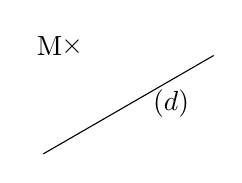
\begin{tikzpicture}[scale=0.5,every node/.style={scale=1},rotate=30]

\draw (0,2) node [left]{M};
\draw (0,2) node {$\times$};
\draw (-2,0)--(3,0) node [near end,below] {$(d)$};


\end{tikzpicture} 
 &  %manuel 6e, chapitre G3
\begin{tikzpicture}[scale=0.5,every node/.style={scale=1},rotate=30]

\draw (0,2) node [left]{M};
\draw (0,2) node {$\times$};
\draw (-2,0)--(3,0) node [near end,below] {$(d)$};
\draw [thick](-0.02,4.2)--(-0.02,2.45);

%%%%%%%%%%%%%%%%%%%%%%%%
%%%%%%%%%%%%%%%%%%%%%%%%
%Définition des paramètres de l'équerre
%et de son positionnement
%%%%%%%%%%%%%%%%%%%%%%%%
%%%%%%%%%%%%%%%%%%%%%%%%

\def \xorigine {0}; %abscisse de l'origine de l'équerre posée avec un xshift
\def \yorigine {0}; %ordonnée de l'origine de l'équerre posée avec un yshift
\def \rotation {0}; %angle de rotation de l'équerre
\def \longueur {4}; %longueur de l'équerre
\def \largeur {2}; %largeur de l'équerre
\def \epaisseur {\longueur * 0.1}; %épaisseur de la partie «colorée» de l'équerre

%%%%%%%%%%%%%%%%%%%%%%%%
%%%%%%%%%%%%%%%%%%%%%%%%
%Tracé de l'équerre
%%%%%%%%%%%%%%%%%%%%%%%%
%%%%%%%%%%%%%%%%%%%%%%%%

\begin{scope}[scale=1.1,xshift=\xorigine cm,yshift=\yorigine cm,rotate=\rotation]

%contour extérieur de l'équerre
\coordinate (A) at (0,0) ; %«origine» de l'équerre
\coordinate (B) at (\largeur,0) ;
\coordinate (C) at (0,\longueur) ;
\draw [gray](A)--(B)--(C)--cycle;


%contour intérieur de l'équerre
\coordinate (D) at (\epaisseur,\epaisseur) ;
\coordinate (E) at ($\largeur*(1,0)-{\largeur * \epaisseur / \longueur}*(1,0)-\epaisseur*(1,0)+\epaisseur*(0,1)$);
\coordinate (F) at ($\epaisseur*(1,0)+\longueur*(0,1)-{2*\longueur * \epaisseur / \largeur}*(0,1)$);
\draw [gray](D)--(E)--(F)--cycle;

%partie colorée de l'équerre
\fill [color=blue!50!gray,opacity=.4,even odd rule] (A)--(B)--(C)--cycle (D)--(E)--(F)--cycle;%l'option even odd rule permet de faire le remplissage entre les 2 zones définies
\end{scope}

%%%%%%%%%%%%%%%%%%%%%%%%
%%%%%%%%%%%%%%%%%%%%%%%%
%Fin de l'équerre
%%%%%%%%%%%%%%%%%%%%%%%%
%%%%%%%%%%%%%%%%%%%%%%%%


%%%%%%%%%%%%%%%%%%%%%%%%
%%%%%%%%%%%%%%%%%%%%%%%%
%Début crayon
%%%%%%%%%%%%%%%%%%%%%%%%
%%%%%%%%%%%%%%%%%%%%%%%%

\begin{scope}[scale=0.35,xshift=0cm,yshift=7cm,rotate=-70] %le crayon, xshift et yshift pour les coordonnées de la pointe, rotate pour l'orientation du crayon
\def \couleur {black}
\coordinate (O) at (0,0);
\fill[\couleur!40] (-0.2,4.8) -- (0.2,4.8) -- (0.2,0.8) --(0.1,0.65) -- (0,0.8) -- (-0.1,0.66) -- (-0.2,0.8) -- cycle; %corps du crayon
\draw[color=white] (0,4.8) -- (0,0.8); %trait intérieur du crayon
\fill[\couleur!90] (-0.2,4.3) -- (0,4.27) -- (0.2,4.3) -- (0.2,4.8) arc(30:150:0.23cm); %partie haute du crayon
\fill[brown!40] (-0.2,0.8) -- (O)node[coordinate,pos=0.75](a){} -- (0.2,0.8)node[coordinate,pos=0.25](b){} -- (0.1,0.65) -- (0,0.8) -- (-0.1,0.66) -- cycle; %pointe du crayon (partie taillée)
\fill[\couleur!90] (a) -- (O) -- (b) -- cycle; %mine du crayon
\end{scope}

%%%%%%%%%%%%%%%%%%%%%%%%
%%%%%%%%%%%%%%%%%%%%%%%%
%Fin crayon
%%%%%%%%%%%%%%%%%%%%%%%%
%%%%%%%%%%%%%%%%%%%%%%%%


\end{tikzpicture} 
 & %manuel 6e, chapitre G3
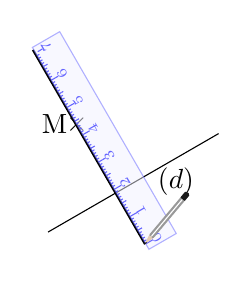
\begin{tikzpicture}[scale=0.5,every node/.style={scale=1},rotate=30]

\draw (0,2) node [left]{M};
\draw (0,2) node {$\times$};
\draw (-2,0)--(3,0) node [near end,below] {$(d)$};
\draw [thick](-0.02,4.2)--(-0.02,-1.5);

%%%%%%%%%%%%%%%%%%%%%%%%
%%%%%%%%%%%%%%%%%%%%%%%%
%Début règle
%%%%%%%%%%%%%%%%%%%%%%%%
%%%%%%%%%%%%%%%%%%%%%%%% 

    %Graduaton max. de la règle
    \def \Taille {7}
    %Définition de l 'angle de rotation de la règle
    \def \Rotation {90}
    %Définition du décalage de la règle
    \def \DecalX {0.4}
    \def \DecalY {-1.5}
    %Couleur des élèments de la règle (sauf le remplissage)
    \def \RegleColor {blue!60}

\begin{scope}[shift={(\DecalX,\DecalY)},rotate=\Rotation,scale=0.8]
    % contours de la règle
    \draw[color=\RegleColor, fill =blue!5, opacity=0.5] (-0.2,0.5) rectangle (\Taille+0.2,-0.5);	%Dont couleur de remplissage
    % graduation 1 mm
    \foreach \a in {0,0.1,...,\Taille}{\draw[color=\RegleColor] (\a,0.5)--(\a,0.42);}
    % graduation 5 mm
    \foreach \a in {0,0.5,...,\Taille}{\draw[color=\RegleColor] (\a,0.42)--(\a,0.35);}
    % graduation et repères 10 mm
    \foreach \a in {0,1,...,\Taille}{\draw[color=\RegleColor] (\a,0.35)--(\a,0.25)
    node[font=\tiny, rotate=\Rotation+30] (\a) at (\a,0.1){\a};}
\end{scope}

%%%%%%%%%%%%%%%%%%%%%%%%
%%%%%%%%%%%%%%%%%%%%%%%%
%Fin de la règle
%%%%%%%%%%%%%%%%%%%%%%%%
%%%%%%%%%%%%%%%%%%%%%%%%

%%%%%%%%%%%%%%%%%%%%%%%%
%%%%%%%%%%%%%%%%%%%%%%%%
%Début crayon
%%%%%%%%%%%%%%%%%%%%%%%%
%%%%%%%%%%%%%%%%%%%%%%%%

\begin{scope}[scale=0.35,xshift=-0.1cm,yshift=-4.28cm,rotate=-70] %le crayon, xshift et yshift pour les coordonnées de la pointe, rotate pour l'orientation du crayon
\def \couleur {black}
\coordinate (O) at (0,0);
\fill[\couleur!40] (-0.2,4.8) -- (0.2,4.8) -- (0.2,0.8) --(0.1,0.65) -- (0,0.8) -- (-0.1,0.66) -- (-0.2,0.8) -- cycle; %corps du crayon
\draw[color=white] (0,4.8) -- (0,0.8); %trait intérieur du crayon
\fill[\couleur!90] (-0.2,4.3) -- (0,4.27) -- (0.2,4.3) -- (0.2,4.8) arc(30:150:0.23cm); %partie haute du crayon
\fill[brown!40] (-0.2,0.8) -- (O)node[coordinate,pos=0.75](a){} -- (0.2,0.8)node[coordinate,pos=0.25](b){} -- (0.1,0.65) -- (0,0.8) -- (-0.1,0.66) -- cycle; %pointe du crayon (partie taillée)
\fill[\couleur!90] (a) -- (O) -- (b) -- cycle; %mine du crayon
\end{scope}

%%%%%%%%%%%%%%%%%%%%%%%%
%%%%%%%%%%%%%%%%%%%%%%%%
%Fin crayon
%%%%%%%%%%%%%%%%%%%%%%%%
%%%%%%%%%%%%%%%%%%%%%%%%


\end{tikzpicture} 
  &  %manuel 6e, chapitre G3
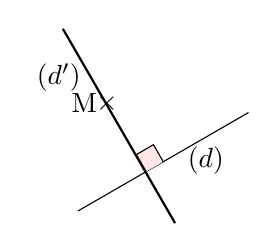
\begin{tikzpicture}[scale=0.5,every node/.style={scale=1},rotate=30]

\draw (0,2) node [left]{M};
\draw (0,2) node {$\times$};
\draw (-2,0)--(3,0) node [near end,below] {$(d)$};
\draw [thick](-0.02,4.2)--(-0.02,-1.5) node[near start,left]{$(d')$};
\draw [fill=pink!40!white](0,0)--(0,0.5)--(0.5,0.5)--(0.5,0);

\end{tikzpicture} 
 \\ 
 On trace une droite $d$ et on place un point $M$. & On place l'un des côtés de l'angle droit de l'équerre sur la droite $d$ et l'autre côté sur $M$.
 & On prolonge la droite à la règle. & On nomme la droite $d'$ et on code l'angle droit par un carré.\\

\end{tabularx} \\
 
 \end{exemple*1}


\exercice

En utilisant cette méthode, tracer un rectangle ABCD de longueur 3 cm et de longueur 5 cm.

%\correction

 
\end{methode*1}

\newpage

%%%%%%%%%%%%%%%%%%%%%%%%%%%%%

\begin{methode*1}[Construire la parallèle à une droite passant par un point]

\begin{exemple*1}
Trace une droite $d$ et place un point $M$ n'appartenant pas à la droite $d$.

Trace la droite $d'$ parallèle à la droite $d$ passant par le point $M$. \\[0.75em]

\begin{tabularx}{1.15\textwidth}{X|X|X|X}
\input{./PointsSegmentsDroites/figures/TracerParal_1}  &  %manuel 6e, chapitre G3
\begin{tikzpicture}[scale=.5,every node/.style={scale=1},rotate=30]

\draw (0,2) node [above left]{M};
\draw (0,2) node {$\times$};
\draw (-2.2,0)--(2.6,0) node [near end,below] {$(d)$};


%%%%%%%%%%%%%%%%%%%%%%%%
%%%%%%%%%%%%%%%%%%%%%%%%
%Définition des paramètres de l'équerre
%et de son positionnement
%%%%%%%%%%%%%%%%%%%%%%%%
%%%%%%%%%%%%%%%%%%%%%%%%

\def \xorigine {-1.65}; %abscisse de l'origine de l'équerre posée avec un xshift
\def \yorigine {0}; %ordonnée de l'origine de l'équerre posée avec un yshift
\def \rotation {-90}; %angle de rotation de l'équerre
\def \longueur {4}; %longueur de l'équerre
\def \largeur {2}; %largeur de l'équerre
\def \epaisseur {\longueur * 0.1}; %épaisseur de la partie «colorée» de l'équerre

%%%%%%%%%%%%%%%%%%%%%%%%
%%%%%%%%%%%%%%%%%%%%%%%%
%Tracé de l'équerre
%%%%%%%%%%%%%%%%%%%%%%%%
%%%%%%%%%%%%%%%%%%%%%%%%

\begin{scope}[scale=.6,xshift=\xorigine cm,yshift=\yorigine cm,rotate=\rotation]

%contour extérieur de l'équerre
\coordinate (A) at (0,0) ; %«origine» de l'équerre
\coordinate (B) at (\largeur,0) ;
\coordinate (C) at (0,\longueur) ;
\draw [gray](A)--(B)--(C)--cycle;


%contour intérieur de l'équerre
\coordinate (D) at (\epaisseur,\epaisseur) ;
\coordinate (E) at ($\largeur*(1,0)-{\largeur * \epaisseur / \longueur}*(1,0)-\epaisseur*(1,0)+\epaisseur*(0,1)$);
\coordinate (F) at ($\epaisseur*(1,0)+\longueur*(0,1)-{2*\longueur * \epaisseur / \largeur}*(0,1)$);
\draw [gray](D)--(E)--(F)--cycle;

%partie colorée de l'équerre
\fill [color=blue!50!gray,opacity=.4,even odd rule] (A)--(B)--(C)--cycle (D)--(E)--(F)--cycle;%l'option even odd rule permet de faire le remplissage entre les 2 zones définies

\end{scope}
%%%%%%%%%%%%%%%%%%%%%%%%
%%%%%%%%%%%%%%%%%%%%%%%%
%Fin de l'équerre
%%%%%%%%%%%%%%%%%%%%%%%%
%%%%%%%%%%%%%%%%%%%%%%%%

%%%%%%%%%%%%%%%%%%%%%%%%
%%%%%%%%%%%%%%%%%%%%%%%%
%Début règle !! Si la figure est tournée, il faut
%rajouter l'angle de rotation dans le node des graduation
%pour que les nombres soient écrits correctement
%%%%%%%%%%%%%%%%%%%%%%%%
%%%%%%%%%%%%%%%%%%%%%%%% 

    %Graduaton max. de la règle
    \def \Taille {5}
    %Définition de l 'angle de rotation de la règle
    \def \Rotation {-90}
    %Définition du décalage de la règle
    \def \DecalX {-1.5}
    \def \DecalY {2.8}
    %Couleur des élèments de la règle (sauf le remplissage)
    \def \RegleColor {blue!60}

\begin{scope}[shift={(\DecalX,\DecalY)},rotate=\Rotation,scale=1]
    % contours de la règle
    \draw[color=\RegleColor, fill =blue!5, opacity=0.5] (-0.2,0.5) rectangle (\Taille+0.2,-0.5);	%Dont couleur de remplissage
    % graduation 1 mm
    \foreach \a in {0,0.1,...,\Taille}{\draw[color=\RegleColor] (\a,0.5)--(\a,0.42);}
    % graduation 5 mm
    \foreach \a in {0,0.5,...,\Taille}{\draw[color=\RegleColor] (\a,0.42)--(\a,0.35);}
    % graduation et repères 10 mm
    \foreach \a in {0,1,...,\Taille}{\draw[color=\RegleColor] (\a,0.35)--(\a,0.25)
    node[font=\tiny, rotate=\Rotation+30] (\a) at (\a,0.1){\a};}%ici rajouter l'angle de rotation de la figure complète pour que les nombres soient écrits correctement
\end{scope}

%%%%%%%%%%%%%%%%%%%%%%%%
%%%%%%%%%%%%%%%%%%%%%%%%
%Fin de la règle
%%%%%%%%%%%%%%%%%%%%%%%%
%%%%%%%%%%%%%%%%%%%%%%%%


\end{tikzpicture} 
 & \input{./PointsSegmentsDroites/figures/TracerParal_3} &  %manuel 6e, chapitre G3
\begin{tikzpicture}[scale=.5,every node/.style={scale=1},rotate=30]

\draw (0,2) node [above left]{M};
\draw (0,2) node {$\times$};
\draw (-2.2,0)--(2.6,0) node [near end,below] {$(d)$};
\draw [red](-1,2)--(0.5,2);

%%%%%%%%%%%%%%%%%%%%%%%%
%%%%%%%%%%%%%%%%%%%%%%%%
%Définition des paramètres de l'équerre
%et de son positionnement
%%%%%%%%%%%%%%%%%%%%%%%%
%%%%%%%%%%%%%%%%%%%%%%%%

\def \xorigine {-1.65}; %abscisse de l'origine de l'équerre posée avec un xshift
\def \yorigine {0}; %ordonnée de l'origine de l'équerre posée avec un yshift
\def \rotation {-90}; %angle de rotation de l'équerre
\def \longueur {4}; %longueur de l'équerre
\def \largeur {2}; %largeur de l'équerre
\def \epaisseur {\longueur * 0.1}; %épaisseur de la partie «colorée» de l'équerre
\def \yorigine2 {3.31}; %ordonnée de l'origine de l'équerre posée avec un yshift

%%%%%%%%%%%%%%%%%%%%%%%%
%%%%%%%%%%%%%%%%%%%%%%%%
%Tracé de l'équerre
%%%%%%%%%%%%%%%%%%%%%%%%
%%%%%%%%%%%%%%%%%%%%%%%%

\begin{scope}[scale=.6,xshift=\xorigine cm,yshift=\yorigine2 cm,rotate=\rotation]

%contour extérieur de l'équerre
\coordinate (A) at (0,0) ; %«origine» de l'équerre
\coordinate (B) at (\largeur,0) ;
\coordinate (C) at (0,\longueur) ;
\draw [gray](A)--(B)--(C)--cycle;


%contour intérieur de l'équerre
\coordinate (D) at (\epaisseur,\epaisseur) ;
\coordinate (E) at ($\largeur*(1,0)-{\largeur * \epaisseur / \longueur}*(1,0)-\epaisseur*(1,0)+\epaisseur*(0,1)$);
\coordinate (F) at ($\epaisseur*(1,0)+\longueur*(0,1)-{2*\longueur * \epaisseur / \largeur}*(0,1)$);
\draw [gray](D)--(E)--(F)--cycle;

%partie colorée de l'équerre
\fill [color=blue!50!gray,opacity=.4,even odd rule] (A)--(B)--(C)--cycle (D)--(E)--(F)--cycle;%l'option even odd rule permet de faire le remplissage entre les 2 zones définies

\end{scope}
%%%%%%%%%%%%%%%%%%%%%%%%
%%%%%%%%%%%%%%%%%%%%%%%%
%Fin de l'équerre
%%%%%%%%%%%%%%%%%%%%%%%%
%%%%%%%%%%%%%%%%%%%%%%%%



%%%%%%%%%%%%%%%%%%%%%%%%
%%%%%%%%%%%%%%%%%%%%%%%%
%Début règle !! Si la figure est tournée, il faut
%rajouter l'angle de rotation dans le node des graduation
%pour que les nombres soient écrits correctement
%%%%%%%%%%%%%%%%%%%%%%%%
%%%%%%%%%%%%%%%%%%%%%%%% 

    %Graduaton max. de la règle
    \def \Taille {5}
    %Définition de l 'angle de rotation de la règle
    \def \Rotation {-90}
    %Définition du décalage de la règle
    \def \DecalX {-1.5}
    \def \DecalY {2.8}
    %Couleur des élèments de la règle (sauf le remplissage)
    \def \RegleColor {blue!60}

\begin{scope}[shift={(\DecalX,\DecalY)},rotate=\Rotation,scale=1]
    % contours de la règle
    \draw[color=\RegleColor, fill =blue!5, opacity=0.5] (-0.2,0.5) rectangle (\Taille+0.2,-0.5);	%Dont couleur de remplissage
    % graduation 1 mm
    \foreach \a in {0,0.1,...,\Taille}{\draw[color=\RegleColor] (\a,0.5)--(\a,0.42);}
    % graduation 5 mm
    \foreach \a in {0,0.5,...,\Taille}{\draw[color=\RegleColor] (\a,0.42)--(\a,0.35);}
    % graduation et repères 10 mm
    \foreach \a in {0,1,...,\Taille}{\draw[color=\RegleColor] (\a,0.35)--(\a,0.25)
    node[font=\tiny, rotate=\Rotation+30] (\a) at (\a,0.1){\a};}%ici rajouter l'angle de rotation de la figure complète pour que les nombres soient écrits correctement
\end{scope}

%%%%%%%%%%%%%%%%%%%%%%%%
%%%%%%%%%%%%%%%%%%%%%%%%
%Fin de la règle
%%%%%%%%%%%%%%%%%%%%%%%%
%%%%%%%%%%%%%%%%%%%%%%%%

%%%%%%%%%%%%%%%%%%%%%%%%
%%%%%%%%%%%%%%%%%%%%%%%%
%Début crayon
%%%%%%%%%%%%%%%%%%%%%%%%
%%%%%%%%%%%%%%%%%%%%%%%%

\begin{scope}[scale=0.3,xshift=1.65cm,yshift=6.65cm,rotate=-70] %le crayon, xshift et yshift pour les coordonnées de la pointe, rotate pour l'orientation du crayon
\def \couleur {black}
\coordinate (O) at (0,0);
\fill[\couleur!40] (-0.2,4.8) -- (0.2,4.8) -- (0.2,0.8) --(0.1,0.65) -- (0,0.8) -- (-0.1,0.66) -- (-0.2,0.8) -- cycle; %corps du crayon
\draw[color=white] (0,4.8) -- (0,0.8); %trait intérieur du crayon
\fill[red] (-0.2,4.3) -- (0,4.27) -- (0.2,4.3) -- (0.2,4.8) arc(30:150:0.23cm); %partie haute du crayon
\fill[brown!40] (-0.2,0.8) -- (O)node[coordinate,pos=0.75](a){} -- (0.2,0.8)node[coordinate,pos=0.25](b){} -- (0.1,0.65) -- (0,0.8) -- (-0.1,0.66) -- cycle; %pointe du crayon (partie taillée)
\fill[red] (a) -- (O) -- (b) -- cycle; %mine du crayon
\end{scope}

%%%%%%%%%%%%%%%%%%%%%%%%
%%%%%%%%%%%%%%%%%%%%%%%%
%Fin crayon
%%%%%%%%%%%%%%%%%%%%%%%%
%%%%%%%%%%%%%%%%%%%%%%%%


\end{tikzpicture} 
\\ 
On trace une droite $d$, on place un point $M$. On place l'un des côtés de l'angle droit de l'équerre sur la droite $d$. & On place la règle le long de l'autre côté de l'équerre & On tient bien la règle et on fait coulisser l'équerre le long de la règle, jusqu'au point $M$. & On trace ainsi la droite $d'$ et on obtient :\vspace{0.3em}
%manuel 6e, chapitre G3
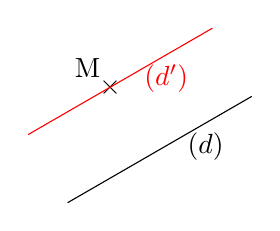
\begin{tikzpicture}[scale=.5,every node/.style={scale=1},rotate=30]

\draw (0,2) node [above left]{M};
\draw (0,2) node {$\times$};
\draw (-2.4,0)--(3,0) node [near end,below] {$(d)$};
\draw [red](-2.4,2)--(3,2) node [near end,below] {$(d')$};

\end{tikzpicture} 
\\
\end{tabularx} \\
 \end{exemple*1}

\exercice

Trace dans ton cahier un segment $[AB]$ d'une longueur de 5 cm et place un point $C$ au-dessus du segment $[AB]$ ($C$ n'est pas sur le segment). Construis, en rouge, la perpendiculaire à $[AB]$ passant par $C$. Construis, en vert, la parallèle à $[AB]$ passant par $C$.
%\correction

\end{methode*1}

\begin{aconnaitre}
\textbf{\underline{Propriété:}}\\
Si deux droites sont parallèles et si une troisième droite est perpendiculaire à l'une d'elle, alors elles est perpendiculaire à l'autre.
\end{aconnaitre}

\begin{methode*1}[Illustration]
\begin{exemple*1}

Soit $(d)$ et $(d')$ deux droites parallèles. Soit $(\Delta)$ un troisième droite.\\
Si $(d)$ et $(\Delta)$ sont perpendiculaires alors $(d')$ et $(\Delta)$ sont également perpendicualires.

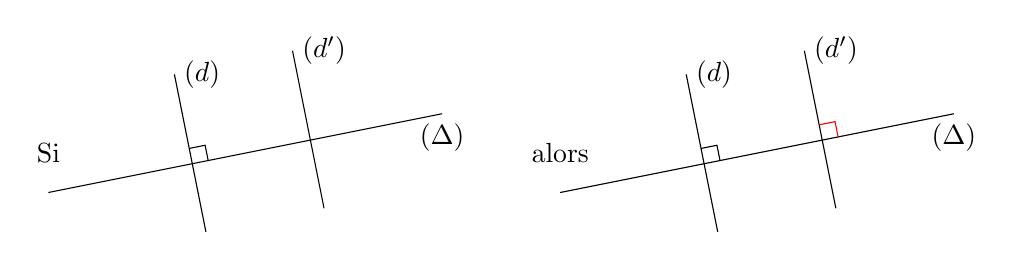
\begin{tikzpicture}
\draw (-2.0,0) node {Si} (-2,-0.5) -- ++(5,1) node[below] {$(\Delta)$} ;
%\draw (-2.0,0) node {Si} (-2,-0.5) ++(1,0.2) -- ++(4,0.8) node[below] {$(\Delta)$} ;
\draw (0,-1) -- ++(-0.4,2) node[right] {$(d)$};
\draw (1.5,-0.7) -- ++(-0.4,2) node[right] {$(d^\prime)$};
\draw (-0.17,-0.14) ++(0.2,0.04) -- ++(-0.04,0.2) -- ++(-0.2, -0.04); %circle (1pt);


\draw (4.5,0) node {alors} ++(0,-0.5) -- ++(5,1) node[below] {$(\Delta)$} ;
\draw (6.5,-1) -- ++(-0.4,2) node[right] {$(d)$};
\draw (8.0,-0.7) -- ++(-0.4,2) node[right] {$(d^\prime)$};
\draw (6.33,-0.14) ++(0.2,0.04) -- ++(-0.04,0.2) -- ++(-0.2, -0.04);
\draw[red] (7.83,0.16) ++(0.2,0.04) -- ++(-0.04,0.2) -- ++(-0.2, -0.04); %circle (1pt);

\end{tikzpicture}
\end{exemple*1}

\exercice

Dans la figure ci-contre:\
\begin{itemize}
\item Tracer la droite $(AB)$.
\item Construire la droite $(d)$ parallèle à $(AB)$ passant par $C$.
\item Construire la droite $(d')$ perpendiculaire à $(AB)$ passant par $B$.
\item Que peut-on dire des droites $(d)$ et $(d')$? Justifier.\\
\end{itemize}
\begin{center}
\tikzset{
   cross/.pic = {
     \draw[thick] (-0.2,0.2) -- (0.2,-0.2);
     \draw[thick] (-0.2,-0.2) -- (0.2,0.2);}
}


\begin{tikzpicture}
\draw (0,0) rectangle (10,6);
\pic[scale=0.6] at (1,3) {cross}; \draw (1,3.5) node {\large $A$};
\pic[scale=0.6] at (6,5) {cross}; \draw (6,5.5) node {\large $B$};
\pic[scale=0.6] at (9,2) {cross}; \draw (9,2.5) node {\large $C$};
\end{tikzpicture}
\end{center}
\end{methode*1}


%%%%%%%%%%%%%%%%%%%%%%%%%%%%%
\newpage

\section{La médiatrice}

\begin{definition}
La \textbf{\MotDefinition{médiatrice}{}} d'un segment est la droite qui coupe ce segment perpendiculairement en son milieu.
\end{definition}


\begin{methode*1}[Construire une médiatrice]

\begin{exemple*1}
Trace un segment $[OS]$ de longueur 5 cm puis sa médiatrice. \\[0.75em]

\begin{tabularx}{\textwidth}{X|X|X|X}
%manuel 6e, chapitre G3

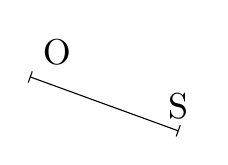
\begin{tikzpicture}[scale=0.5,every node/.style={scale=1.3}]

\def \CharSize {2.5};

\begin{scope}[rotate=-20]
\draw (-2,0)--(2,0);
\draw (-2,0)--+(90:0.15)--+(-90:0.15);
\draw (2,0)--+(90:0.15)--+(-90:0.15);
\node [above right] at (-2,0) {O};
\node [above] at (2,0) {S};
\end{scope}

\end{tikzpicture}  &

% Attention, il faut déclarer la librairie calc :\usetikzlibrary{calc}  pour les calculs de coordonnées des points


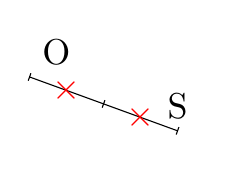
\begin{tikzpicture}	[scale=0.5,every node/.style={scale=1.3}]

\begin{scope}[rotate=-20] %la figure
\draw (-2,0)--(0,0) node [midway,red] {$\times$};
\draw (0,0)--(2,0) node [midway,red] {$\times$};
\draw (-2,0)--+(90:0.1)--+(-90:0.1);
\draw (2,0)--+(90:0.1)--+(-90:0.1);
\draw (0,0)--+(90:0.1)--+(-90:0.1);
\node [above right] at (-2,0) {O};
\node [above] at (2,0) {S};
\end{scope}

\end{tikzpicture} 
 
 & 
% Attention, il faut déclarer la librairie calc :\usetikzlibrary{calc}  pour les calculs de coordonnées des points

\begin{tikzpicture}[scale=0.5,every node/.style={scale=1.3}]
  
%%%%%%%%%%%%%%%%%%%%%%%%
%%%%%%%%%%%%%%%%%%%%%%%%
%Définition des paramètres de l'équerre
%et de son positionnement
%%%%%%%%%%%%%%%%%%%%%%%%
%%%%%%%%%%%%%%%%%%%%%%%%

\def \xorigine {0}; %abscisse de l'origine de l'équerre posée avec un xshift
\def \yorigine {0}; %ordonnée de l'origine de l'équerre posée avec un yshift
\def \rotation {-20}; %angle de rotation de l'équerre
\def \longueur {4}; %longueur de l'équerre
\def \largeur {2}; %largeur de l'équerre
\def \epaisseur {\longueur * 0.1}; %épaisseur de la partie «colorée» de l'équerre

%%%%%%%%%%%%%%%%%%%%%%%%
%%%%%%%%%%%%%%%%%%%%%%%%
%Tracé de l'équerre
%%%%%%%%%%%%%%%%%%%%%%%%
%%%%%%%%%%%%%%%%%%%%%%%%
\begin{scope}[scale=0.8,xshift=\xorigine cm,yshift=\yorigine cm,rotate=\rotation]

%contour extérieur de l'équerre
\coordinate (A) at (0,0) ; %«origine» de l'équerre
\coordinate (B) at (\largeur,0) ;
\coordinate (C) at (0,\longueur) ;
\draw [gray](A)--(B)--(C)--cycle;


%contour intérieur de l'équerre
\coordinate (D) at (\epaisseur,\epaisseur) ;
\coordinate (E) at ($\largeur*(1,0)-{\largeur * \epaisseur / \longueur}*(1,0)-\epaisseur*(1,0)+\epaisseur*(0,1)$);
\coordinate (F) at ($\epaisseur*(1,0)+\longueur*(0,1)-{2*\longueur * \epaisseur / \largeur}*(0,1)$);
\draw [gray](D)--(E)--(F)--cycle;

%partie colorée de l'équerre
\fill [color=blue!50!gray,opacity=0.5,even odd rule] (A)--(B)--(C)--cycle (D)--(E)--(F)--cycle;%l'option even odd rule permet de faire le remplissage entre les 2 zones définies

\end{scope}

\begin{scope}[scale=0.5,xshift=.32cm,yshift=3cm,rotate=30] %le crayon
\fill[gray!50] (0,4) -- (0.4,4) -- (0.4,0) --(0.3,-0.15) -- (0.2,0) -- (0.1,-0.14) -- (0,0) -- cycle;
\draw[color=white] (0.2,4) -- (0.2,0);
\fill[black] (0,3.5) -- (0.2,3.47) -- (0.4,3.5) -- (0.4,4) arc(30:150:0.23cm);
\fill[brown!40] (0,0) -- (0.2,-0.8)node[coordinate,pos=0.75](a){} --(0.4,0) node[coordinate,pos=0.25](b){} -- (0.3,-0.15) -- (0.2,0) -- (0.1,-0.14) -- cycle;
\fill[black] (a) -- (0.2,-0.8) -- (b) -- cycle;
\end{scope}

\begin{scope}[rotate=-20] %la figure
\draw (-2,0)--(0,0) node [midway,red] {$\times$};
\draw (0,0)--(2,0) node [midway,red] {$\times$};
\draw (-2,0)--+(90:0.1)--+(-90:0.1);
\draw (2,0)--+(90:0.1)--+(-90:0.1);
\draw (0,0)--+(90:0.1)--+(-90:0.1);
\node [above right] at (-2,0) {O};
\node [above] at (2,0) {S};

\draw (0,0)--($(0,0)!1.3cm!90:(2,0)$); %trace un segment de 1.3cm à 90° du segment allant de (0,0) à (2,0)

\end{scope}



\end{tikzpicture} 
  &  \input{./PointsSegmentsDroites/figures/Mediatrice4}  \\ 
On trace un segment $[OS]$. & On trace le milieu du segment. & On trace la droite perpendiculaire au segment qui passe par ce milieu. & On code l'angle droit par un carré. \\
\end{tabularx} \\

 \end{exemple*1}
 
 \begin{exemple*1}
Trace un segment $[AB]$ de longueur 6 cm. Construis sa médiatrice au compas. \\[0.75em]

\begin{tabular}{l|l|l|l}
 \textcolor{H1}{\circled{1}} &  \textcolor{H1}{\circled{2}} &  \textcolor{H1}{\circled{3}} & \textcolor{H1}{\circled{1}} On trace le segment $[AB]$. \\ 
 \multirow{7}{*}{

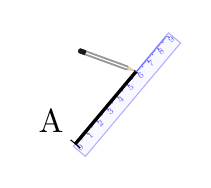
\begin{tikzpicture}[scale=0.2,rotate=50,every node/.style={scale=1.2}]

%début de la règle
    %Graduaton max. de la règle
    \def \Taille {9}
    %Définition de l 'angle de rotation de la règle
    \def \Rotation {0}
    %Définition du décalage de la règle
    \def \DecalX {0}
    \def \DecalY {0}
    %Couleur des élèments de la règle (sauf le remplissage)
    \def \RegleColor {blue!60}

\begin{scope}[scale=1,shift={(\DecalX,\DecalY)},rotate=\Rotation]
    % contours de la règle
    \draw[color=\RegleColor, fill =blue!5, opacity=0.5] (-0.2,0.5) rectangle (\Taille+0.2,-0.5);	%Dont couleur de remplissage
    % graduation 1 mm
    \foreach \a in {0,0.1,...,\Taille}{\draw[color=\RegleColor] (\a,0.5)--(\a,0.42);}
    % graduation 5 mm
    \foreach \a in {0,0.5,...,\Taille}{\draw[color=\RegleColor] (\a,0.42)--(\a,0.35);}
    % graduation et repères 10 mm
    \foreach \a in {0,1,...,\Taille}{\draw[color=\RegleColor] (\a,0.35)--(\a,0.25)
    node[scale=0.5,font=\tiny, rotate=40] (\a) at (\a,0.1){\a};}
%fin de la règle

\draw (0,0.5) node[above left]{A};
\draw (0,0.5)--+(90:0.4)--+(-90:0.4);
\draw [very thick](0,0.5)--(6,0.5);

\end{scope}

\begin{scope}[scale=0.8,xshift=7.52cm,yshift=.62cm,rotate=20] %le crayon, xshift et yshift pour les coordonnées de la pointe, rotate pour l'orientation du crayon
\def \couleur {black}
\coordinate (O) at (0,0);
\fill[\couleur!40] (-0.2,4.8) -- (0.2,4.8) -- (0.2,0.8) --(0.1,0.65) -- (0,0.8) -- (-0.1,0.66) -- (-0.2,0.8) -- cycle; %corps du crayon
\draw[color=white] (0,4.8) -- (0,0.8); %trait intérieur du crayon
\fill[\couleur!90] (-0.2,4.3) -- (0,4.27) -- (0.2,4.3) -- (0.2,4.8) arc(30:150:0.23cm); %partie haute du crayon
\fill[brown!40] (-0.2,0.8) -- (O)node[coordinate,pos=0.75](a){} -- (0.2,0.8)node[coordinate,pos=0.25](b){} -- (0.1,0.65) -- (0,0.8) -- (-0.1,0.66) -- cycle; %pointe du crayon (partie taillée)
\fill[\couleur!90] (a) -- (O) -- (b) -- cycle; %mine du crayon
\end{scope}


\end{tikzpicture}


} &  \multirow{7}{*}{

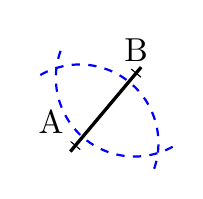
\begin{tikzpicture}[scale=0.2,rotate=50,every node/.style={scale=1.2}]

\draw [very thick](-0.5,0.5)--(6.5,0.5);
\draw (0,0.5)--+(90:0.4)--+(-90:0.4);
\draw (6,0.5)--+(90:0.4)--+(-90:0.4);
\draw (0,0.5) node[above left]{A};
\draw (6,0.5) node[above]{B};

\draw [style=dashed,color=blue,thick](4,5.083) arc (110:250:5);
\draw [style=dashed,color=blue,thick](2,5.083) arc (70:-70:5);
%\draw (3,6)--(3,-6);

\coordinate (A) at (0,0.5) ;
\coordinate (B) at (2,5.083) ;
\begin{scope}[scale=.8]
\Compas{A}{B}
\end{scope}

\end{tikzpicture}
} & \multirow{7}{*}{

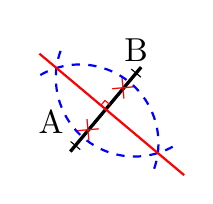
\begin{tikzpicture}[scale=0.2,rotate=50,every node/.style={scale=1.2}]

%\draw [very thick](-0.5,0.5)--(6.5,0.5);
\draw [very thick](-0.5,0.5)--(3,0.5) node[midway,red,rotate=50]{$\times$}--(6.5,0.5)node[midway,red,rotate=50]{$\times$};
\draw (0,0.5)--+(90:0.4)--+(-90:0.4);
\draw (6,0.5)--+(90:0.4)--+(-90:0.4);
\draw (0,0.5) node[above left]{A};
\draw (6,0.5) node[above]{B};

\draw [style=dashed,color=blue,thick](4,5.083) arc (110:250:5);
\draw [style=dashed,color=blue,thick](2,5.083) arc (70:-70:5);
\draw [thick,color=red](3,6)--(3,-6);
\draw [color=red](3,0.9)-|(3.4,0.5);

\end{tikzpicture}
} &  \textcolor{H1}{\circled{2}} On trace deux arcs de cercle\\ % exemple de fusion de cellules d'une même colonne
&&& de centres $A$ et $B$, de même\\ 
&&& rayon, en choisissant un\\
&&& rayon suffisamment grand\\
&&& pour que ces arcs se coupent\\
&&&  en deux points.\\ 
&&& \textcolor{H1}{\circled{3}} La médiatrice de [AB] est \\
&&&  la droite qui passe par ces\\
&&& deux points.\\ 
\end{tabular} \\

 \end{exemple*1}

\exercice 
Trace un segment $[AB]$ de 7 cm. Trace la médiatrice du segment $[AB]$ par la méthode de ton choix.
%\correction

 
\end{methode*1}

%%%%%%%%%%%%%%%%%%%%%%%%%%%%%


\section{Les angles}

%%%%%%%%%%%%%%%%%%%%%%%%%%%%%

% remarque : pour qu'un mot se retrouve dans le lexique : \MotDefinition{asymptote horizontale}{} 

\begin{definition}
Un \MotDefinition{angle}{} est une portion de plan délimitée par deux demi-droites ayant la même origine.
 \end{definition}

\subsection{Reconnaître les différents types d'angles}

On classe les angles par catégories selon leur mesure.

 \renewcommand*\tabularxcolumn[1]{>{\centering\arraybackslash}m{#1}}
 \begin{ttableau}{\linewidth}{6}
\hline \textbf{Angle} 	&	Nul	&	Aigu		&	Droit		&	Obtus	&	Plat	\\ \hline
 \textbf{Figure} 	&	\includegraphics[width=1.7cm]{angle_nul}	&	\includegraphics[width=1.7cm]{angle_aigu}	&	\includegraphics[width=1.7cm]{angle_droit}	&	\includegraphics[width=1.7cm]{angle_obtus}	&	\includegraphics[width=1.7cm]{angle_plat}	\\ \hline
 \textbf{Mesure} 	&	$0^\circ$	&	entre $0^\circ$ et $90^\circ$	&	$90^\circ$		&	entre $90^\circ$ et $180^\circ$	&	 $180^\circ$	\\ \hline
 \multirow{3}{*}{} \textbf{Position} 	&		&	&	&	&	dans le 	\\ 
 \textbf{des}	&	confondus		&	&	perpendiculaires	&	&	 prolongement	\\
\textbf{côtés}	&	&	&	&	&	 l'un de l'autre	\\ \hline
 \end{ttableau}

%%%%%%%%%%%%%%%%%%%%%%%%%%%%%

\begin{methode*1}[Nommer un angle]

\begin{exemple*1}
Nomme l'angle marqué en violet sur la figure ci‑dessous.  \\[0.75em]

\begin{minipage}[c]{0.70\textwidth}
Le sommet de l'angle est le point $C$ : c'est la lettre centrale. \\[0.5em]
Les côtés de l'angle sont les demi‑droites $[CH)$ (ou $[Cx)$) et $[CS)$ (ou $[CA)$ (ou $[Cy)$). \\[0.5em]
Cet angle peut se nommer : $\widehat{{\textcolor{A1}{H}}C{\textcolor{C1}{S}}}$; $\widehat{{\textcolor{C1}{S}}C{\textcolor{A1}{H}}}$ ; $\widehat{{\textcolor{A1}{H}}C{\textcolor{C1}{A}}}$ ; $\widehat{{\textcolor{C1}{A}}C{\textcolor{A1}{H}}}$ ; $\widehat{{\textcolor{C1}{y}}C{\textcolor{A1}{x}}}$.
 \end{minipage} \hfill%
 \begin{minipage}[c]{0.26\textwidth}
 \includegraphics[width=3.8cm]{nommer_angle}
 \end{minipage} \\
 
\end{exemple*1}

\exercice 
Nomme les angles marqués sur la figure ci‑dessous. 
\begin{center} \includegraphics[width=4.5cm]{nommer_angles} \end{center}
%\correction
 
\end{methode*1}

%%%%%%%%%%%%%%%%%%%%%%%%%%%%%

\begin{methode*1}[Utiliser le rapporteur]

\begin{exemple*1}
Mesure l'angle $\widehat{CAB}$. \\[0.75em]

\begin{minipage}[c]{0.49\textwidth}
\centering
\includegraphics[width=4.8cm]{rapporteur1}
\end{minipage}\hfill%
 \begin{minipage}[c]{0.49\textwidth}%
 \centering
 \includegraphics[width=6.6cm]{rapporteur2}
  \end{minipage} \\
 \begin{minipage}[c]{0.43\textwidth}
On place le centre du rapporteur sur le sommet de l'angle.
\end{minipage} \hfill%
 \begin{minipage}[c]{0.53\textwidth}
 On place un zéro du rapporteur sur le côté $[AC)$. Si besoin, on prolonge la demi‑droite $[AC)$. La mesure de l'angle est donnée par l'autre côté de l'angle sur \underline{la même échelle} de graduation.
 \end{minipage} \\
  \end{exemple*1}
 
 \begin{exemple*1}
Construis un angle $\widehat{BUT}$ de $108^\circ$.  \\[0.75em]

\begin{minipage}[c]{0.49\textwidth}
\centering
\includegraphics[width=4.8cm]{rapporteur3}
\end{minipage}\hfill%
 \begin{minipage}[c]{0.49\textwidth}%
 \centering
 \includegraphics[width=6.6cm]{rapporteur44}
  \end{minipage} \\
 \begin{minipage}[c]{0.43\textwidth}
On trace $[UB)$, premier côté de l'angle. On place le centre du rapporteur sur le point $U$.
\end{minipage} \hfill%
 \begin{minipage}[c]{0.53\textwidth}
 On place un zéro du rapporteur sur le côté $[UB)$. On marque, d'un petit trait-repère, $108^\circ$ avec la bonne graduation.
On trace la demi‑droite d'origine $U$ passant par le repère. On place un point $T$ sur cette demi‑droite.
  \end{minipage} \\
  \end{exemple*1}
 
\exercice
 \begin{enumerate}
 \begin{minipage}[c]{0.36\textwidth}
  \item Mesure l'angle $\widehat{xOy}$ ci‑contre ;
  \item Construis un angle $\widehat{SAT}$ de $85^\circ$. 
  \end{minipage} \hfill%
 \begin{minipage}[c]{0.56\textwidth}
  \includegraphics[width=6cm]{angleyOx} 
  \end{minipage} \\
  \end{enumerate}
%\correction
 
\end{methode*1}

%%%%%%%%%%%%%%%%%%%%%%%%%%%%%


\section{La bissectrice}

\begin{definition}
La \textbf{\MotDefinition{bissectrice}{}} d'un angle est la demi-droite qui a pour origine le sommet de l'angle et qui partage l'angle en deux angles de même mesure.
\end{definition}


\begin{methode*1}[Construire une bissectrice]


\begin{exemple*1} \\[0.75em]
Trace un angle $\widehat{xOy}$. Construis sa bissectrice au compas. \\[0.5em]

\begin{tabularx}{\textwidth}{X|X|X}
 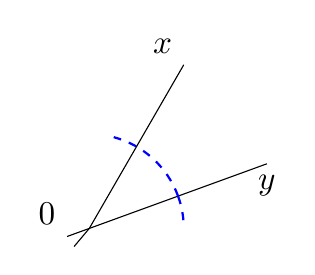
\begin{tikzpicture}[scale=0.6,rotate=20,every node/.style={scale=1.2}]

\draw (-0.5,0) node[above left]{0}--(4,0) node[below]{$y$};
\draw (0,0) --(40:4) node[above left]{$x$};
\draw (0,0)--+(210:0.5);
\draw[thick,dashed,blue] (2,0) arc (0:55:2);
\draw[thick,dashed,blue] (2,0) arc (0:-15:2);

\coordinate (A) at (0,0) ;
\coordinate (B) at (1.414,1.414) ;


\begin{scope}[scale=0.35]
\Compas{A}{B}
\end{scope}


\end{tikzpicture}

 &  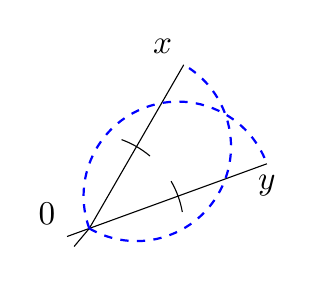
\begin{tikzpicture}[scale=0.6,rotate=20,every node/.style={scale=1.2}]

\draw (-0.5,0) node[above left]{0}--(4,0) node[below]{$y$};
\draw (0,0) --(40:4) node[above left]{$x$};
\draw (0,0)--+(210:0.5);

\draw (1.532,1.286) arc (40:50:2);
\draw (1.532,1.286) arc (40:30:2);
\draw (2,0) arc (0:10:2);
\draw (2,0) arc (0:-10:2);

\draw [thick,blue,dashed](0,0) arc (180:0:2);
\draw [thick,blue,dashed](0,0) arc (-140:40:2);

%\draw (2,0) node{$\bullet$};
%\draw (1.532,1.286) node{$\bullet$};
%\draw (0,0)--(4.698,1.71);

\coordinate (A) at (1.532,1.286) ;
\coordinate (B) at (3.064,2.572) ;

\begin{scope}[scale=0.35]
\Compas{A}{B}
\end{scope}


\end{tikzpicture}

 & 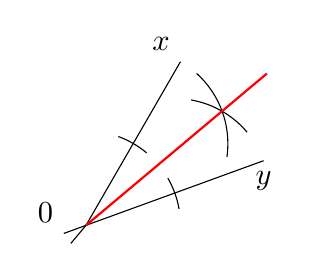
\begin{tikzpicture}[scale=0.6,rotate=20,every node/.style={scale=1.1}]

\draw (-0.5,0) node[above left]{0}--(4,0) node[below]{$y$};
\draw (0,0) --(40:4) node[above left]{$x$};
\draw (0,0)--+(210:0.5);

\draw (1.532,1.286) arc (40:50:2);
\draw (1.532,1.286) arc (40:30:2);
\draw (2,0) arc (0:10:2);
\draw (2,0) arc (0:-10:2);
\draw (3,1.732) arc (60:20:2);
\draw (3.3,2.221) arc (28:-28:2);

\draw [red,thick](0,0)--(4.698,1.71);


\end{tikzpicture}

 \\ 
Au compas, on trace un arc de cercle de centre $O$ qui coupe chaque côté de l'angle en un point. & On trace deux arcs de cercle de même rayon ayant ces deux points pour centres. Ces arcs se coupent en un point. & La bissectrice de l'angle $\widehat{xOy}$ est la demi-droite d'origine $O$ passant par ce point. \\
\end{tabularx} \\

 \end{exemple*1}

\exercice 

Trace un triangle $ABC$ tel que $AB=4$\,cm ; $AC=7$\,cm ; $BC=5$\,cm ; puis trace les bissectrices des angles $\widehat{ABC}$ ; $\widehat{BAC}$ et $\widehat{ACB}$. Que remarques-tu ?

%\correction

 
\end{methode*1}

%%%%%%%%%%%%%%%%%%%%%%%%%%%%%

%%%%%%%%Mise en page
\newpage
%%%%%%%%%%%%%%%%%%%%



\section{Le cercle}

\begin{definition}
Un \textbf{\MotDefinition{cercle}{}} de centre $O$ est l'ensemble des points situés à la même distance du point $O$. 
Cette distance est le \textbf{\MotDefinition{rayon}{}} du cercle.
\end{definition}

\begin{aconnaitre}
\begin{tabularx}{.95\linewidth}{|X|p{5cm}|p{3cm}|}
\hline
\multirow{5}{*}{\includegraphics[width=3.4cm]{cercleAFNME}}  & Le \textcolor{C2}{\textbf{centre}} d'un cercle est le point équidistant de tous les points qui constituent ce cercle. & Le point $O$ est le \textcolor{C2}{\textbf{centre}} du cercle $(\mathcal{C})$.\\ \cline{2-3}
 & Un \textcolor{J1}{\textbf{rayon}} d'un cercle est un segment ayant pour extrémités le centre et un point de ce cercle. & Le segment $[OA]$ est un  \textcolor{J1}{\textbf{rayon}} du cercle $(\mathcal{C})$.\\ \cline{2-3}
  & Un  \textcolor{H1}{\textbf{diamètre}} d'un cercle est un segment ayant pour extrémités deux points de ce cercle et contenant son centre. & Le segment $[EF]$ est un  \textcolor{H1}{\textbf{diamètre}} du cercle $(\mathcal{C})$.\\ \cline{2-3}
 & Une  \textcolor{PartieFonction}{\textbf{corde}} d'un cercle est un segment ayant pour extrémités deux points de ce cercle. & Le segment $[MN]$ est une  \textcolor{PartieFonction}{\textbf{corde}} du cercle $(\mathcal{C})$.\\ \cline{2-3}
 & Un  \textcolor{B2}{\textbf{arc de cercle}} est une portion de cercle comprise entre deux points de ce cercle. & La portion de cercle $\overset{\huge{\frown}}{MN}$ comprise entre $M$ et $N$ est un  \textcolor{B2}{\textbf{arc du cercle}} $(\mathcal{C})$.\\ \hline
  \end{tabularx}
 \end{aconnaitre}
  
  
 \begin{remarque}
 Par commodité de langage, on appelle « rayon » la longueur du rayon d'un cercle, et  on appelle « diamètre » la longueur de son diamètre.
  \end{remarque}
  
 \begin{remarque}
 Le diamètre d'un cercle est égal au double de son rayon.
  \end{remarque}